\documentclass[a4paper]{article}
\usepackage{algorithmic}
\usepackage{array}
\usepackage{url,amsfonts,amsmath,amssymb,amsthm,color,enumerate,tikz,hyperref}
\usepackage{algorithm,bbm}
\usepackage{mathtools}
% \usepackage{indentfirst}
\usepackage{stackrel}
\usepackage{listings}
\usepackage{subfigure}
\usepackage{subfloat}
\usepackage[justification=centering]{caption}
\usepackage{booktabs} % for three-line table
% \usepackage{subfig}
\usepackage{graphicx}
\setcounter{tocdepth}{4}
\setcounter{secnumdepth}{4}

\hyphenation{op-tical net-works semi-conduc-tor}
\usetikzlibrary{shapes, shadows, arrows}
% \usepackage[english]{babel}
% \usepackage[utf8]{inputenc}
% \usepackage{amsmath}
% \usepackage{graphicx}
% \usepackage[colorinlistoftodos]{todonotes}

\title{Mathematical Model of Input for Peak-Detector}

\author{Author}

\date{\today}

% def some function
\DeclarePairedDelimiter\ceil{\lceil}{\rceil}
\DeclarePairedDelimiter\floor{\lfloor}{\rfloor}

\begin{document}

% \author{Yu Wang% <-this % stops a space
% % \thanks{}% <-this % stops a space
% }

% The paper headers
% \markboth{}%
% {}
\maketitle
\tableofcontents
\newpage
% \IEEEpeerreviewmaketitle
\section{Introduction} % (fold)
\label{sec:Introduction}
CDMA system is famous for its large user capacity and superior ability of keeping security. In practical CDMA system, the diagram of the whole system is like 
\begin{figure}[ht]
	\centering
	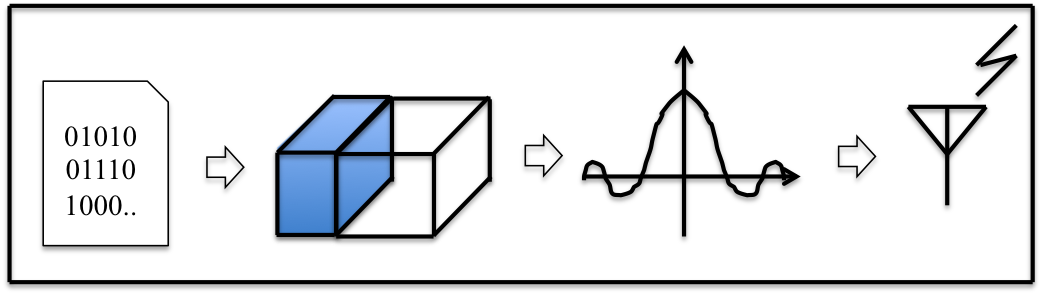
\includegraphics[width=3.1in]{figure/tx.png}
	\caption{TX model}
	\label{fig:TX diagram}
	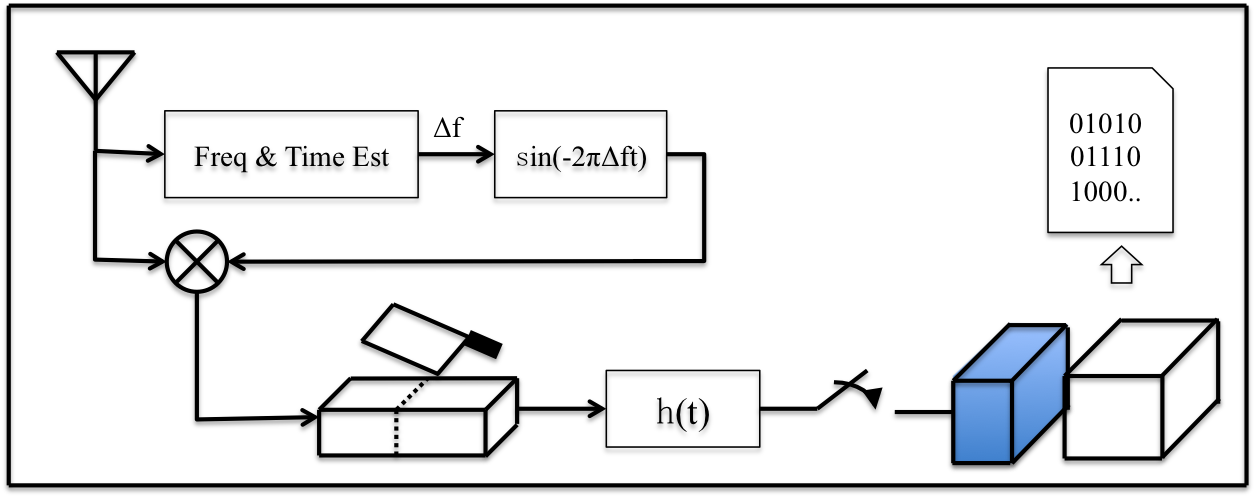
\includegraphics[width = 3.1in]{figure/rx.png}
	\caption{RX model}
	\label{fig:RX diagram}
\end{figure}

From the diagrams, we can see that the complexity of RX model is much more complicated then TX model. The reason is that, the channel will add several uncertainty to the signal, while the transmitter doesn't have to deal with that. So, the main block in the RX model is the ``freq\_\&time\_est'', which will give out the frequency and timing information of the received signal. This article is mainly focus on the performance of this block. 
% section Introduction (end)

\section{Frequency and TIming Trade-off in Estimation}

Trade-off is common in the world. There is one famous theory called uncertainty principle\cite{Uncertainty_Principle}. Also, there is also a trade off for estimating frequency and timing.

In this scenario, we are trying to estimate the frequency offset of the received signal, and estimate the start point of the frame. We will prove that, the estimation cannot be perfect.

\subsection{Mathematical Model} % (fold)
\label{sub:mathematical_model}
The signal we use is $s(t)$:
\begin{align}
	s(t) = 
	\begin{cases}
		\alpha & 0 \leq t \leq T_s\\
		0 	   & else
	\end{cases}
\end{align}
This is a very simple rectangle wave.
For the receiver, we only consider about delay $t_0$ and frequency offset $\Delta f$, the received signal $r(t)$ would be
\begin{align}
	r(t) = s(t - t_0) e^{j 2 \pi \Delta f t}
\end{align}
But for the receiver, it doesn't know anything about the receiver, so the only tag receiver could choose for the matched filter is $h(t)$
\begin{align}
	h(t) = s(T_s - t)
\end{align}
Then, the output of the matched filter is $R(t)$, the result of convolution between $r(t)$ and $h(t)$. 
\begin{align}
	R(t) = r(t) \ast h(t) 
	&= \int_{-\infty}^{+\infty} r(\tau) h(t - \tau) d\tau\\
	&= \int_{t_0}^t s(\tau - t_0)e^{j 2 \pi \Delta f \tau} s(\tau - (t - T_s)) d \tau\\
	&= \int_{t_0}^t \alpha^2 e^{j 2 \pi \Delta f \tau} d \tau\\
	&= \alpha^2 \frac{e^{j 2 \pi \Delta f t}}{j 2\pi \Delta f} \bigg|_{t_0}^t\\
	&= \alpha^2 \frac{e^{j 2\pi \Delta f t} - e^{j 2\pi \Delta f t_0}}{j 2\pi \Delta f}
\end{align}

Now, we will discuss three specific situations:
\subsubsection{$\Delta f = 0$ and $t_0 = 0$} % (fold)
\label{ssub:no freq offset or delay}
We will find that, the numerator and denominator are all 0, so we will turn to L'Hospital.
\begin{align}
	 &\lim_{\Delta f \rightarrow 0} \alpha^2 \frac{e^{j 2\pi \Delta f t} - e^{j 2\pi \Delta f t_0}}{j 2\pi \Delta f}\\
	 =& \lim_{\Delta f \rightarrow 0} \alpha^2 \frac{j 2\pi t e^{j 2\pi \Delta f t} - j 2\pi t_0 e^{j 2\pi \Delta f t_0}}{j 2\pi}\\
	 =& \alpha^2(t - t_0)
\end{align}
When $t_0 = 0$, $R(t) = \alpha^2 t$.
And we know that, because of the domain of $t$, we know that, when $t = T_s$, $R(t)$ will get its maximum value $R(Ts) = \alpha^2 T_s$.

\subsubsection{$\Delta f = 0$, $t_0 = ?$} % (fold)
\label{ssub:no freq offset, but delay is unknown}
Similar to the procedure in part \ref{ssub:no freq offset or delay}, also sample at $t = T_s$
\begin{align}
	R(t) = \alpha^2(T_s-t_0) \Rightarrow \hat{t_0} = T_s - \frac{R(t)}{\alpha^2}
\end{align}

\subsubsection{$t_0 = 0$, but $\Delta f = ?$} % (fold)
\label{ssub:no delay, but freq offset is unknown}
Sample at $t = T_s$
\begin{align}
	R(t) = \alpha^2 \frac{e^{j 2\pi \Delta f T_s} - 1}{j 2\pi \Delta f} = \alpha^2 T_s e^{j \pi \Delta f T_s} sa(\Delta 2 \pi f Ts)
\end{align}
So, we know that, when we get the correct $\Delta f$, we will get the largest value. 

But we still haven't touch the situation where $\Delta f = ?$ and $t_0 = ?$. Our method is brute search.
We enumerate all the possible pair of parameters $(t_0', \Delta f')$, and try them. With the help of above three theory, we know that, the correct/similar to true value will give out the largest $R(t)$.
% subsection mathematical_model (end)

\section{Input Signal of Peak Detector} % (fold)
\label{sec:input_signal_of_peak_detector}
For the ``freq\_timing\_est'' block, frequency and timing information are supposed to be estimated. As discussed in the ``freq\_timing\_tradeoff'', we can use brutal search to get the correct value. But, before we make our decision by choosing the maximum peak, we still need to have a rigorous mathematic model for the peak. 

This section will discuss the mathematic model for ``True'' peak and other points.


\subsection{Mathematical Model} % (fold)
\label{sub:mathematical_model}
Because the signal we received are discrete values, so we only consider about discrete signals, rather than continuous ones.

\begin{table}[ht]
\centering
\begin{tabular}{l l}
 \toprule
 Notation 	& 	Description\\
 \midrule
 $s_k$		& 	received sample at time $k$\\
 $t_k$		& 	training sample at time $k$\\
 $d_k$		& 	data sample at time $k$\\
 $n_k$		& 	noise at time $k$\\
 $P^t_k$ & 	the $k^{th}$ chip of spread code for one frame of training\\
 $P^d_k$	& 	the $k^{th}$ chip of spread code for one frame of data\\
 $D^t_l$ & 	the $l^{th}$ symbol for training\\
 $D^d_l$ & 	the $l^{th}$ symbol for data\\
 $N_f$ 		& 	number of chips per frame\\
 $N_c$ 		& 	number of chips per symbol\\
 $N_s$		& 	number of symbols per frame\\
 $N_{s'}$ 	& 	number of symbols per shortened training sequence\\
 $\sigma^2$ & 	variance of Gaussian noise\\
 $k_0$ 		& 	number of samples of delay\\
 $f_0$ 		& 	frequency offset\\
 $T_c$ 		& 	duration between two chips\\
 \bottomrule
\end{tabular}
\caption{Notation Table}
\label{Table:Notation Table}
\end{table}

First, the structure of training and data frame are like:
The structure of training is like Fig. \ref{fig:Training Frame Structure} and Fig. \ref{fig:Data Frame Structure}
\begin{figure}[ht]
	\centering
	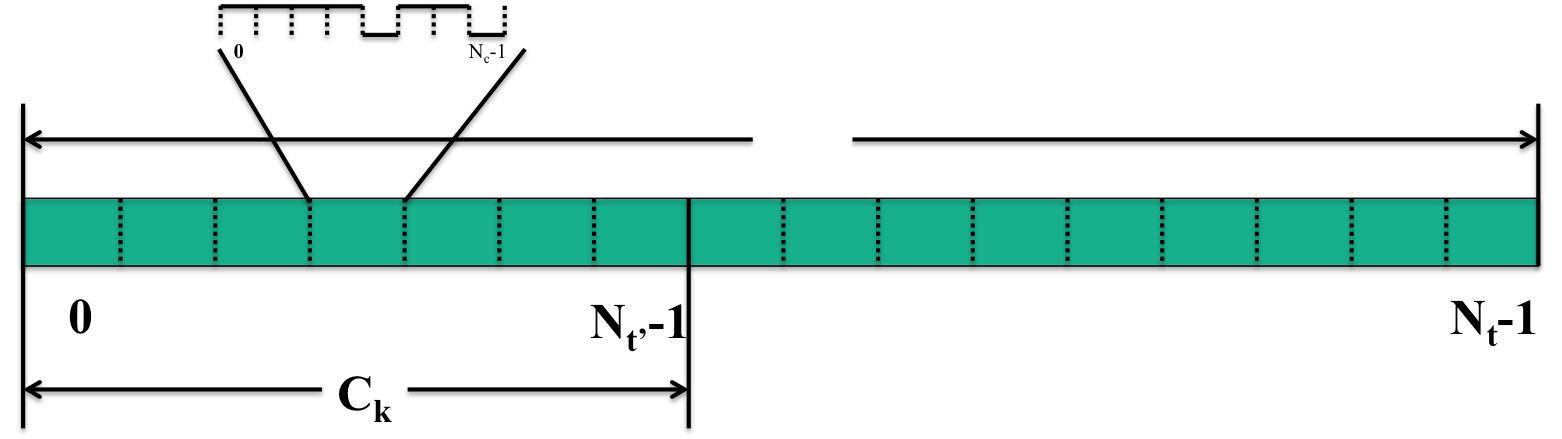
\includegraphics[width = 3.1in]{figure/training_frame.png}
	\caption{Training Frame Structure}
	\label{fig:Training Frame Structure}
	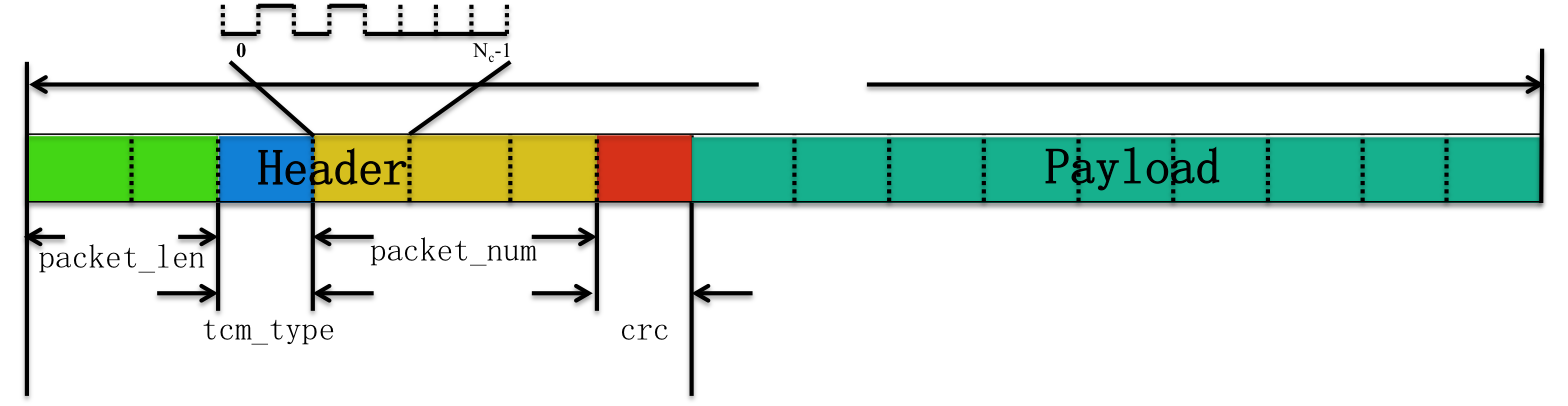
\includegraphics[width = 3.1 in]{figure/data_frame.png}
	\caption{Data Frame Structure}
	\label{fig:Data Frame Structure}
\end{figure}

\subsubsection{Description of Variables} % (fold)
\label{ssub:description_of_variables}
We first express each variables by mathematical languages.

According to the description in table \ref{Table:Notation Table}, and also in order to simplify the following notation, the definition of $P^x_y$ is defined as 
\begin{equation}
\begin{split}
	&P^x_k = 
	\begin{cases}
		P^x_k 	& k = 0, \cdots, N_c-1\\
		0 			& else
	\end{cases}\\
	&x = ``t'' or ``d''
\end{split}
\end{equation}

For instance, the figure for $P^t_k$ is like Fig. \ref{fig:Sketch Map of P_tk}
\begin{figure}
	\centering
	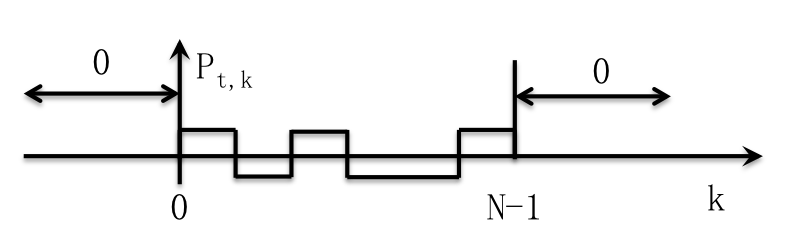
\includegraphics[width = 3.1 in]{figure/p_t_k.png}
	\caption{Sketch Map of $P^t_k$}
	\label{fig:Sketch Map of P_tk}
\end{figure}

So, training chip at time $k$ can be described as:
\begin{align}
		t_k 
	&= \sum_{k = 0}^{N_c} D^t_0 P^t_{k}\\
	&= D^t_0 P^t_k \label{eq:t_k only consider the cyclic property of symbol level}
\end{align}

If we consider the frame-level periodicity, $t_k$ would be
\begin{align}
	t_k = D^t_{\floor{k / N_c} \% N_s} P^t_{k \% N_c}
\end{align}

Based on nearly the same idea, $d_k$ can be written as:
\begin{align}
	d_k = D^d_{\floor{k / N_c}} P^d_{k \% N_c}
\end{align}

Noise is simple. We simply choose IID Gaussian noise. So
\begin{align}
	n_k \sim \mathcal{N}(0, \sigma^2)
\end{align}
% subsubsection description_of_variables (end)

\subsubsection{Description of Output of Matched Filter} % (fold)
\label{ssub:description_of_output_of_matched_filter}
Consider the time delay and frequency offset, the received signal would be 
\begin{align}
	r_k = (t_{k - k_0} + d_{k - k_0}) e^{j 2\pi f_0 k T_c} + n_k
\end{align}

We first deal with the contribution of noise.
Define the Pulse Response of Matched Filter to be $h_{N_f-k}$.
\begin{align}
	h_k = 
	\begin{cases}
	P^t_{k} = D^t_{\floor{k/N_c}}P^t_{k\%N_c} & k = 0, \cdots, N_f\\
	0 	& else	
	\end{cases}
\end{align}
Let $g^n_{k_0}= \sum_{k' = 0}^{N_f-1} n_{k'} \cdot h_{k'}$

\begin{align}
	\mathbb{E} \{ g^n_{k_0}\}
	&= \mathbb{E} \{\sum_{k' = 0}^{N_f-1} n_{k'} \cdot h_{k'}\} \\
	&= \sum_{k' = 0}^{N_f-1} \mathbb{E} \{ n_{k'} \cdot h_{k'} \} \\
	&= \sum_{k' = 0}^{N_f-1} \mathbb{E} \{ n_{k'}\} h_{k'} \\
	&= \sum_{k' = 0}^{N_f-1} 0 \cdot h_{k'} \\
	&= 0\\
	\mathbb{E} \{ (g^n_{k_0})^2\}
	&= \mathbb{E} \{\sum_{k' = 0}^{N_f-1} (n_{k'} \cdot h_{k'}\} \\
	&= \mathbb{E} \{\sum_{k' = 0}^{N_f-1} n_{k'}^2 \cdot \underbrace{(h_{k'})^2}_{\equiv1}\} \\
	&= \sum_{k' = 0}^{N_f-1} \mathbb{E} \{n_{k'}^2 \}\\
	&= N_f \sigma^2
\end{align}

So $g^n_{k_0}\sim \mathcal{N} (0, N_f \sigma^2)$

The next step is to analyze the output of Matched Filter. 
Define the patten for Matched Filter for training frame to be $P^{t*}_{-k}$.
The output of the Matched Filter at sampled point $k=N_f$ is:
\begin{align}
	g_{k_0} 
	&= r_k \ast h_{N_f - k} \bigg|_{k = N_f-1}\\
	&= (t_{k - k_0} + d_{k - k_0} + n_k) \ast h_{N_f -1- k} \bigg|_{k = N_f-1}\\
	&= \underbrace{\sum_{k' = 0}^{N_f-1} t_{k'-k_0}\cdot h_{k'}}_{g^t_{k_0}} + \underbrace{\sum_{k' = 0}^{N_f-1} d_{k'-k_0}\cdot h_{k'}}_{g^d_{k_0}} + \underbrace{\sum_{k' = 0}^{N_f-1} n_{k'}\cdot h_{k'}}_{g^n_{k_0}}\\
	&= g^t_{k_0} + g^d_{k_0} + g^n_{k_0}
	% g_{k_0}
	% &= r_k \ast h_{N_f-k} \bigg|_{k = N_f}\\
	% &= \sum_{k' = 0}^{N_f-1} r_{k'} h_{N_f-(k - k')}\bigg|_{k = N_f}\\
	% &= \sum_{k' = k-N_f+1}^{k} r_{k'} \cdot h_{k' + (N_f-k)}\bigg|_{k = N_f}\\
	% &= \sum_{k' = 0}^{N_f-1} (t_{k'-k_0-N_f+1} + d_{k'-k_0-N_f+1} + n_{k'-k_0-N_f+1}) \cdot h_{k'}\\
	% &= \sum_{k' = 0}^{N_f-1} (t_{k'-k_0-N_f+1} + d_{k'-k_0-N_f+1}) \cdot h_{k'} + \sum_{k' = 0}^{N_f-1} n_{k'-k_0-N_f+1} \cdot h_{k'}\\
	% &= \sum_{k' = 0}^{N_f-1} (t_{k'-k_0-N_f+1} + d_{k'-k_0-N_f+1}) \cdot h_{k'} + \sum_{k' = 0}^{N_f-1} n_{k'} \cdot h_{k'}\\
	% &= \sum_{k' = 0}^{N_f-1}  (t_{k'-k_0-N_f+1} + d_{k'-k_0-N_f+1}) \cdot h_{k'} + g^n_{k}\\
	% &= \underbrace{\sum_{k' = 0}^{N_f-1} t_{k'-k_0-N_f+1} \cdot h_{k'}}_{g^t_{k_0}} + \underbrace{\sum_{k' = 0}^{N_f-1} d_{k'-k_0-N_f+1} \cdot h_{k'}}_{g^d_{k_0}} + g^n_{k_0}\\
	% &= g^t_{k_0}+ g^d_{k_0}+ g^n_{k_0}
\end{align}

Now, we will discuss all the possible situations for timing. 
Let's formate the time offset $k_0$ in terms of $N_s$ and $N_c$.
\begin{align}
	k_0 = \alpha \cdot N_c + \beta ~~~ \alpha = \mathbb{Z}~and~\beta = 0, \cdots, N_c - 1
\end{align}


\paragraph{Perfectly Aligned} % (fold)
\label{par:perfectly_aligned}
Perfectly Aligned means the sample at time $k$ is also the first sample of patten for Matched Filter, as shown in fig. \ref{fig:Perfectly Aligned}.
\begin{figure}[ht]
	\centering
	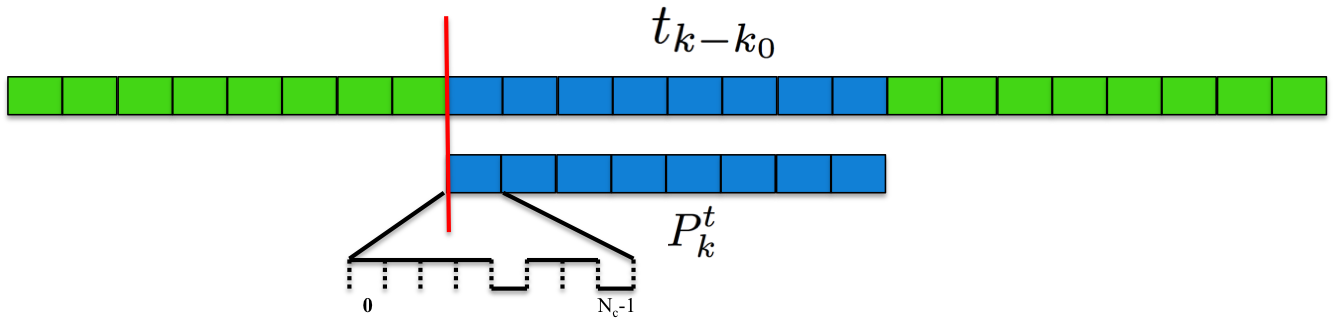
\includegraphics[width=3.1in]{figure/perfectly_aligned.png}
	\caption{Perfectly Aligned}
	\label{fig:Perfectly Aligned}
\end{figure}
For this situation, $k_0$ satisfies 
\begin{align}
	\begin{cases}
		\alpha = z \cdot N_s ~ z \in \mathbb{Z}\\
		\beta = 0
	\end{cases}
	\Rightarrow
	k_0 = z \cdot N_s \cdot N_c
\end{align}

Then we can analyze $g^t_{k_0}$ and $g^d_{k_0}$ separately.

For $g^t_{k_0}$: \label{eq:perfectly aligned-training}
\begin{align}
	g^t_{k_0}
	&= \sum_{k' = 0}^{N_f-1} t_{k'-k_0} \cdot h_{k'}\\
	&= \sum_{k' = 0}^{N_f-1} D^t_{\floor{(k'-k_0) / N_c}\%N_s} P^t_{k' \% N_c} \cdot h_{k'}\\
	&= \sum_{k' = 0}^{N_f-1} D^t_{\floor{(k'-z \cdot N_s \cdot N_c) /N_c}\% N_s} P^t_{k' \% N_c} \cdot h_{k'}\\
	&= \sum_{k' = 0}^{N_f-1} D^t_{\floor{k'/N_c}\%N_s} P^t_{k' \% N_c} \cdot h_{k'}\\
\end{align}
\begin{align}
	\because 
	h_{k'} &= D^t_{\floor{k'/N_c}} P^t_{k' \% N_c}\\
	\therefore
	g^t_{k_0}
	&= \sum_{k' = 0}^{N_f-1} D^t_{\floor{k'/N_c}\%N_s} P^t_{k' \% N_c} \cdot D^t_{\floor{k'/N_c}} P^t_{k \% N_c} \\
	&= \sum_{k' = 0}^{N_f-1} \underbrace{(D^t_{\floor{k'/N_c}\%N_s})^2}_{\equiv 1} \underbrace{(P^t_{k' \% N_c})^2}_{\equiv1}\\
	&= N_f
\end{align}

To analyzie $g^s_k$, we will first define a function to describe the convolution
\begin{align}
	C^n_s(f_1, f_2, k_0) = \sum_{k = s}^{s+n} f_1(k)\cdot f_2(k - k_0) \label{eq:New Defined Convolution}
\end{align}

The diagram of the above formula is like Fig.\ref{fig:New Defined Convolution}
\begin{figure}[ht]
	\centering
	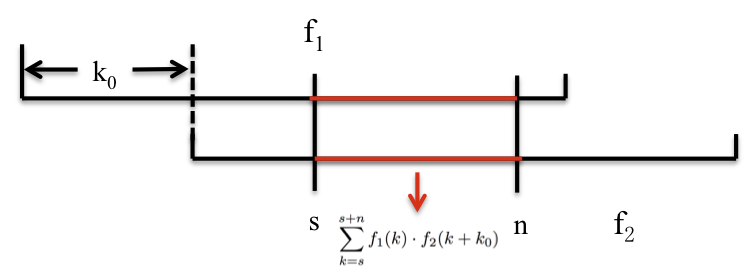
\includegraphics[width=3.1in]{figure/conv_figure.png}
	\caption{New Defined Convolution}
	\label{fig:New Defined Convolution}
\end{figure}
Then $g^d_{k_0}$: \label{eq:perfectly aligned-data}
\begin{align}
	g^d_{k_0}
	&= \sum_{k' = 0}^{N_f-1} d_{k' - k_0} \cdot h_{k'} \\
	&= \sum_{k' = 0}^{N_f-1} D^d_{\floor{(k' - k_0)/N_c}}P^d_{(k' - k_0)\%N_c} \cdot h_{k'}\\
	&= \sum_{k' = 0}^{N_f-1} D^d_{\floor{(k' - z \cdot N_s \cdot N_c)/N_c}} P^d_{(k' - z \cdot N_s \cdot N_c)\%N_c}\cdot h_{k'}\\
	&= \sum_{k' = 0}^{N_f-1} D^d_{\floor{k'/N_c} - z \cdot N_s} P^d_{k'\%N_c} \cdot D^t_{\floor{k'/N_c}} P^t_{k' \% N_c} 
\end{align}
For data symbols, we could only assume that 
\begin{align}
	D^d_k = 
	\begin{cases}
	+1 & p = 0.5\\
	-1 & p = 0.5	
	\end{cases}
\end{align}
Because the $D^d_k$ here is a random variable, we could only exam the mean and variance for it, so do the $g^d_{k_0}$
\begin{align}
	&\mathbb{E} \{D^d_k\} = 1 \times 0.5 + (-1) \times 0.5 = 0\\
	&\mathbb{E} \{D^d_k)^2\} = 1 \times 0.5 + (-1)^2 \times 0.5 = 1
\end{align}
and they are IID.

For $g^d_{k_0}$,

\begin{align}
	% mean
	\mathbb{E} \{g^d_{k_0}\} 
	&= \mathbb{E} \{\sum_{k' = 0}^{N_f-1} D^d_{\floor{k'/N_c} - z \cdot N_s} P^d_{k'\%N_c} \cdot D^t_{\floor{k'/N_c}} P^t_{k' \% N_c}\}\\
	&= \sum_{k' = 0}^{N_f-1} \mathbb{E}\{ D^d_{\floor{k'/N_c} - z \cdot N_s} P^d_{k'\%N_c} \cdot D^t_{\floor{k'/N_c}} P^t_{k' \% N_c}\}\\
	&= \sum_{k' = 0}^{N_f-1} P^d_{k'\%N_c} P^t_{k' \% N_c} \mathbb{E} \{ D^d_{\floor{k'/N_c} - z \cdot N_s} D^t_{\floor{k'/N_c}}\}\\
	&= C_0^{N_c-1}(P^d_{k}, P^t_{k}, 0) \sum_{k'' = \floor{k'/N_c}}^{\floor{k'/N_c} + N_s - 1} D^t_{k''}\mathbb{E} \{ D^d_{k'' - z} \}\\
	&= 0
\end{align}
\begin{align}
	% variance
	\mathbb{E} \{(g^d_{k_0})^2\}
	&= \mathbb{E} \{\sum_{k' = 0}^{N_f-1} D^d_{\floor{k'/N_c} - z \cdot N_s} P^d_{k'\%N_c} \cdot D^t_{\floor{k'/N_c}\%N_s} P^t_{k \% N_c}\}^2\\
	&= \mathbb{E} \{\sum_{k'' = \floor{k'/N_c}}^{\floor{k'/N_c} + N_s - 1} D^t_{k''} D^d_{k'' - z} \cdot \sum_{m = 0}^{N_c} P^d_{m\%N_c} P^t_{m \% N_c} \}^2\\
	&= \big(\sum_{m = 0}^{N_c} P^d_{m} P^t_{m }\big)^2 \mathbb{E} \{\sum_{k'' = \floor{k'/N_c}}^{\floor{k'/N_c} + N_s - 1} D^t_{k''} D^d_{k'' - z}\}^2\\
	&= (C_0^{N_c-1}(P^d_{k}, P^t_{k}, 0))^2 \mathbb{E}\{\sum_{k'' = \floor{k'/N_c}}^{\floor{k'/N_c} + N_s - 1} D^t_{k''} D^d_{k''}\}^2\\ 
	\begin{split}
		&=(C_0^{N_c-1}(P^d_{k}, P^t_{k}, 0))^2 \bigg(\mathbb{E} \{\sum_{m = \floor{k'/N_c}}^{\floor{k'/N_c} + N_s - 1} (D^t_{m} D^d_{m})^2\}\\
		&+ \mathbb{E} \{ \sum_{m = \floor{k'/N_c}}^{\floor{k'/N_c} + N_s - 1} \sum_{n \neq m} D^t_{m} D^d_{m} D^t_{n} D^d_{n}\} \bigg)
	\end{split}\\
	\begin{split}
		&= (C_0^{N_c-1}(P^d_{k}, P^t_{k}, 0))^2 \bigg( \sum_{m = \floor{k'/N_c}}^{\floor{k'/N_c} + N_s - 1} \mathbb{E} \{ D^d_{m}\}^2\\
		&+ \sum_{m = \floor{k'/N_c}}^{\floor{k'/N_c} + N_s - 1} \sum_{n \neq m} D^t_{m} D^t_{n} \mathbb{E} \{D^d_{m}\} \mathbb{E} \{D^d_{n}\} \bigg)
	\end{split}\\
	&= (C_0^{N_c-1}(P^d_{k}, P^t_{k}, 0))^2 \bigg( \sum_{m = \floor{k'/N_c}}^{\floor{k'/N_c} + N_s - 1} \cdot 1 \bigg)\\
	&= (C_0^{N_c-1}(P^d_{k}, P^t_{k}, 0))^2 \cdot N_s
\end{align}
% paragraph perfectly_aligned (end)


% paragraph  (end)
\paragraph{Chip-level Aligned} % (fold)
\label{par:chip_level_aligned}
Chip-level Aligned means the start chip of received symbol is aligned with patten's symbol's first chip. But, the begining symbol of a frame for received data may not be aligned with patten's first symbol. Here is the diagram
\begin{figure}[ht]
	\centering
	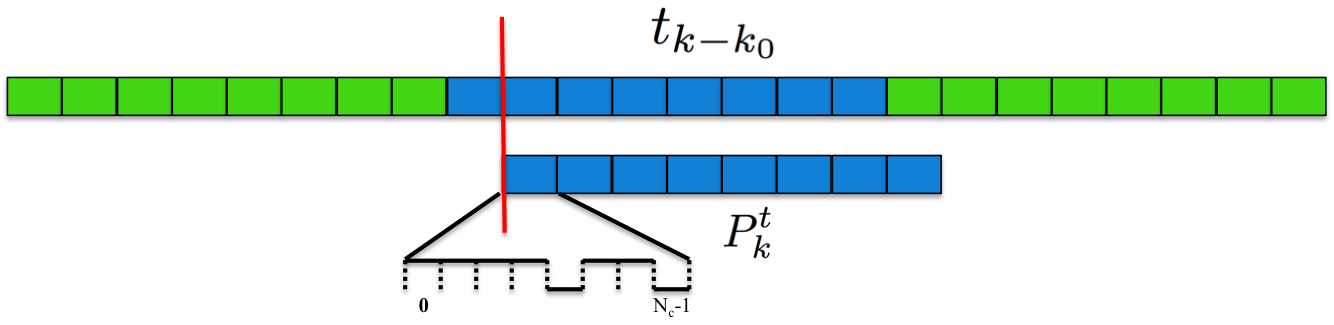
\includegraphics[width = 3.1in]{figure/chip_level_aligned.png}
	\caption{Chip-level Aligned}
	\label{fig:Chip-level aligned}
\end{figure}

At this time
\begin{align}
	\begin{cases}
		\alpha = z &z \in \mathbb{Z}\\
		\beta = 0 &
	\end{cases}
	\Rightarrow k_0 = z \cdot N_c
\end{align}

For $g^t_{k_0}$: \label{eq:chip-level aligned-training}
\begin{align}
	g^t_{k_0}
	&= \sum_{k' = 0}^{N_f-1} t_{k'-k_0} \cdot h_{k'}\\
	&= \sum_{k' = 0}^{N_f-1} D^t_{\floor{(k'-k_0) / N_c}\%N_s} P^t_{k \% N_c} \cdot h_{k'}\\
	&= \sum_{k' = 0}^{N_f-1} D^t_{\floor{(k'-z \cdot N_c) / N_c}\%N_s} P^t_{k \% N_c} \cdot D^t_{\floor{k'/N_c}} P^t_{k \% N_c}\\
	&= \sum_{k' = 0}^{N_f-1} D^t_{(\floor{k' / N_c} - z)\%N_s} D^t_{\floor{k'/N_c}} \underbrace{P^t_{k \% N_c} P^t_{k \% N_c}}_{\equiv 1}\\
	&= \sum_{k' = 0}^{N_f-1} D^t_{(\floor{k' / N_c} - z)\%N_s} D^t_{\floor{k'/N_c}}\\
	&= C_z^{N_s-1}(D_k^t, D_k^t, z) + C_{N_s - z}^{N_s-1}(D_k^t, D_k^t, N_s - z)
\end{align}
\begin{figure}[ht]
	\centering
	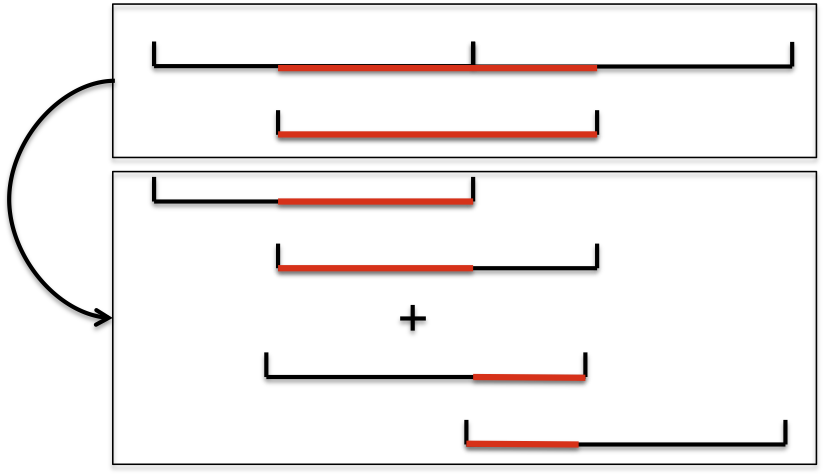
\includegraphics[width=3.1in]{figure/misaligned_conv.png}
	\caption{Diagram for Misaligned Convolution}
	\label{fig:Diagram for Misaligned Convolution}
\end{figure}

For $g^d_{k_0}$: \label{eq:chip-level aligned-data}
\begin{align}
	% mean
	\mathbb{E} \{g^d_{k_0}\} 
	&= \mathbb{E} \{\sum_{k'=0}^{N_f-1} D^d_{\floor{k'/N_c}-z} P^d_{k'\%N_c} \cdot D^t_{\floor{k'/N_c}\%N_s} P^t_{k\%N_c} \}\\
	&= \sum_{k'=0}^{N_f-1} \mathbb{E} \{ D^d_{\floor{k'/N_c}-z} P^d_{k'\%N_c} \cdot D^t_{\floor{k'/N_c}\%N_s} P^t_{k\%N_c} \}\\
	&= \sum_{m = 0}^{N_c} (P^d_{m} P^t_{m}) \sum_{m = \floor{k'/N_c}}^{\floor{k'/N_c}+N_s-1} D^t_{m} \mathbb{E}\{ D^d_{m-z} \}\\
	&= C_0^{N_c}(P_k^d, P_k^t, 0) \cdot \sum_{m = \floor{k'/N_c}}^{\floor{k'/N_c}+N_s-1} D^t_{m} \cdot0\\
	&= 0
\end{align}
\begin{align}
	% variance
	\mathbb{E} \{(g^d_{k_0})^2\}
	&= \mathbb{E} \{\sum_{k'=0}^{N_f-1} D^d_{\floor{k'/N_c}-z} P^d_{k'\%N_c} \cdot D^t_{\floor{k'/N_c}\%N_s} P^t_{k\%N_c} \}^2\\
	&= (C_0^{N_c}(P_k^d, P_k^t, 0))^2 \mathbb{E}\{\sum_{m = \floor{k'/N_c}}^{\floor{k'/N_c}+N_s-1} D_{m-z}^t D_{m}^d \}^2\\
	&= (C_0^{N_c}(P_k^d, P_k^t, 0))^2 \mathbb{E}\{\sum_{m = \floor{k'/N_c}}^{\floor{k'/N_c}+N_s-1} D_{m}^t D_{m}^d \}^2\\
	&= (C_0^{N_c-1}(P^d_{k}, P^t_{k}, 0))^2 \cdot N_s
\end{align}

The mean and variance of $g^d_{k_0}$ is the same as the situation of perfectly aligned.
% paragraph chip_level_aligned (end)

\paragraph{Totally Misaligned} % (fold)
\label{par:totally_misaligned}
Totally Misaligned means the first chip of received data is not correspond to the first chip of patten. Like the Fig. \ref{fig:Totally Misaligned}
\begin{figure}[ht]
	\centering
	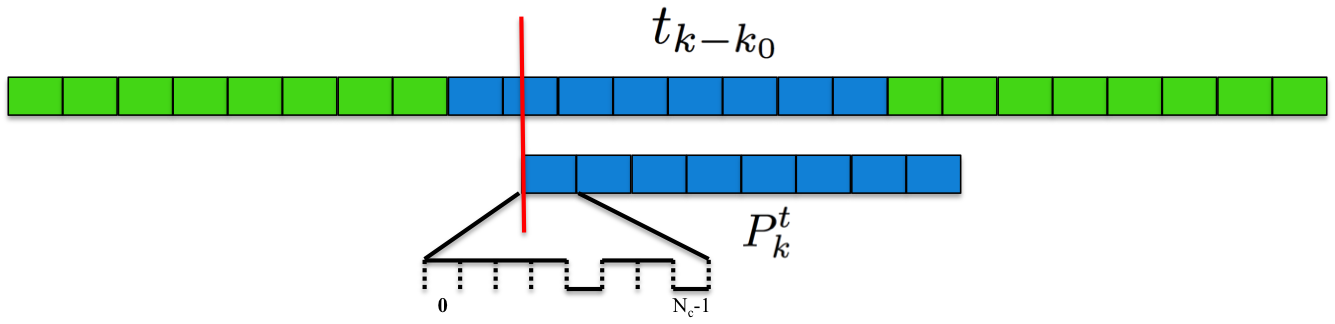
\includegraphics[width = 3.1in]{figure/totally_misaligned.png}
	\caption{Totally Misaligned}
	\label{fig:Totally Misaligned}
\end{figure}

\begin{align}
	k_0 = z, ~ z\in \mathbb{Z}
\end{align}

For $g_{k_0}^t$: \label{eq:totally misaligned-training}
\begin{align}
	g^t_{k_0} 
	&= \sum_{k' = 0}^{N_f-1} t_{k' - k_0} \cdot h_{k'}\\
	&= \sum_{k' = 0}^{N_f-1} D^t_{\floor{(k'-z)/N_c}\%N_s} P^t_{(k'-z)\% N_c} \cdot D^t_{\floor{k'/N_c}} P^t_{k\%N_c}
\end{align}

We will first deal with a smaller problem. If we only focus on patten of length $N_c$
\begin{figure}[ht]
	\centering
	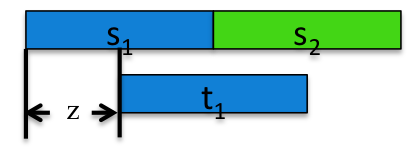
\includegraphics[width = 3.1in]{figure/chip_level_misaligned.png}
	\caption{Chip-level Misaligned}
	\label{Chip-level Misaligned}
\end{figure}
Define the result of the above situation to be $f^t(s_1, s_2, t_1, z)$
\begin{align}
	f^t(s_1, s_2, t_1, z) = (s_1 \cdot t_1)C_z^{N_c-1}(P^t_{k}, P^t_{k}, z) + (s_2 \cdot t_1) C_{N_c - z}^{N_c-1}(P^t_{k}, P^t_{k}, N_c - z)
\end{align}
Now, back to $g^t_{k_0}$ \label{eq:totally misaligned-training}
\begin{align}
	g^t_{k_0}
	&= \sum_{m = \floor{(-k_0)/N_c}, n = 0}^{\floor{m=(-k_0)/N_c} + N_s, n = N_s} f^t_{m\%N_s, m+1\%N_s, n, z\%N_c}
\end{align}

For $g^d_{k_0}$ \label{eq:totally misaligned-data}
\begin{align}
	\mathbb{E} \{g^d_{k_0}\} 
	&= \sum_{k' = 0}^{N_f-1} D^d_{\floor{(k'-z)/N_c}\%N_s} P^d_{(k'-z)\% N_c} \cdot D^t_{\floor{k'/N_c}} P^t_{k\%N_c}
\end{align}

We can also define
\begin{align}
	f^d_1(s_1, s_2, t_1, z) = (s_1 \cdot t_1)C_z^{N_c-1}(P^d_{k}, P^t_{k}, z) + (s_2 \cdot t_1) C_{N_c - z}^{N_c-1}(P^d_{k}, P^t_{k}, N_c - z)
\end{align}

Then $g_{k_0}^d$ would be 
\begin{align}
	g^d_{k_0}
	&= \sum_{m = \floor{(-k_0)/N_c}, n = 0}^{\floor{m=(-k_0)/N_c} + N_s, n = N_s} f^d(m, m+1, n, z\%N_c)
\end{align}
But for the expectation, we may need to change a little bit. Because we want to split the patten symbol rather than the received symbol.
\begin{align}
	g^d_{k_0}
	&= \sum_{m = \floor{(-k_0)/N_c}, n = 0}^{\floor{m=(-k_0)/N_c} + N_s, n = N_s} f^d(n, n+1, m, z\%N_c)
\end{align}
Then
\begin{align}
	\mathbb{E}\{g^d_{k_0}\} 
	&= \mathbb{E}\{\sum_{m = \floor{(-k_0)/N_c}, n = 0}^{\floor{m=(-k_0)/N_c} + N_s, n = N_s} f^d(n, n+1, m, z\%N_c)\}\\
	&= \sum_{m = \floor{(-k_0)/N_c}, n = 0}^{\floor{m=(-k_0)/N_c} + N_s, n = N_s} \mathbb{E}\{f^d(n, n+1, m, z\%N_c)\}\\
	&= 0
\end{align}
\begin{align}
	\mathbb{E} \{(g^d_{k_0})^2\}
	&= \bigg(C_{z\%N_c}^{N_c-1}(P^d_k, P^t_k, z\%N_c) + C_0^{z-1}(P^d_k, P^t_k, -z\%N_c)\bigg)^2 \cdot N_s
\end{align}

Because we can view it as a shifted training patten.


\subsubsection{Ideal Situation} % (fold)
\label{ssub:ideal_situation}

The formulas above are for practical situations. For idea situations, we would like to let spread codes have properities like below:

\begin{enumerate}
	\item Different spread codes are orthogonal;
	\item Autocorrelation is a $\delta$ function.
\end{enumerate}

So the auto-correlation and cross-correlation are like:

\begin{figure}[ht]
	\centering
	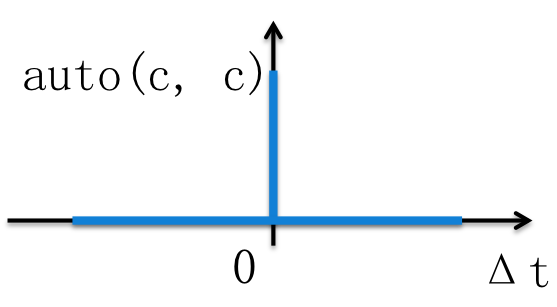
\includegraphics[width = 3.1in]{figure/autocorrelation.png}
	\caption{Auto-correlation for certain spread codes}
	\label{fig:auto-correlation}
	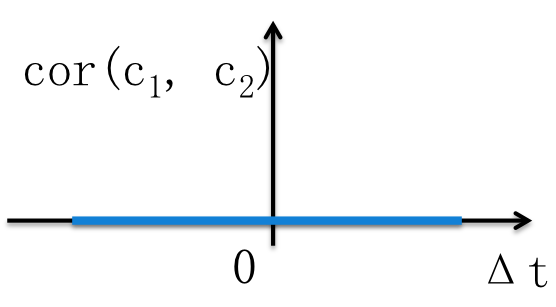
\includegraphics[width = 3.1in]{figure/cross-correlation.png}
	\caption{Cross-correlation for different spread codes}
	\label{fig:cross-correlatino}
\end{figure}

The mathematical description for this property would be:
\begin{align}
	&\text{for different spread codes }C_i(t) \text{and} C_j(t), i \neq j \text{means they are different.} \nonumber\\
	&c_i(t) \ast c_i(-t + \Delta t) = 
	\begin{cases}
		N_c &	\Delta t = k \cdot N_c, k = \mathbb{Z}\\
		0 	& 	else
	\end{cases}\\
	&c_i(t) \ast c_j(-t + \Delta t) = 0, \forall k \in \mathbb{Z}
\end{align}

Compared the ideal situation with the analysis did in subsection \ref{ssub:description_of_output_of_matched_filter}, because the spread code for training and data are orthogonal, or say different, so 

\begin{align}
	g^d_{k_0} \equiv 0
\end{align}

Because the auto-correlation function has perfect property, eq \ref{eq:chip-level aligned-training} and eq \ref{eq:totally misaligned-training} should be as close to 0 as possible.
% subsubsection ideal_situation (end)

% paragraph input_signal_of_peak_detector (end)





\bibliographystyle{plain}
\bibliography{bibliography.bib}




\end{document}